\section{Experimental Setup}
\label{sec:setup}
In order to see whether explanations are helpful in detecting biases of the training data we used the publicly available housing price data~\cite{housing} and created a version that has a bias that needs to be detected.
Originally a regression task, we converted the data set into a classification task predicting whether the house price is above \$150k (598 instances above; 433 instances below; 1031 instances in total).
We also reduced the number of features in the data set to 10 in order to make it possible to see all features at once in all conditions, without the need to scroll, so data otherwise hidden off-screen would not be a confounding effect.
The biased dataset needed to have a bias detectable in both the aggregated and instance-level version, thus we chose to manipulate the outcome of the biased data set to be dependent on the value of one feature (``Living Area'') with some random perturbations.
The biased outcome was chosen so that a \emph{larger} ``Living Area'' results in a \emph{lower} house price.
This relationship does not reflect reality (an increased ``Living Area'' generally results in a higher house price).
The bias is present to the same degree in both the training and the testing data.

Furthermore, by controlling the degree of randomness while creating the biased data set we controlled the accuracy of the prediction when training a machine learning model, such that the model using the biased data has a \emph{higher} accuracy than the model on the real data.
We trained Multi-Layer Perceptrons~\cite{mlp} on both data sets resulting in test accuracies of $81.96\%$ for the real data and $88.33\%$ for the biased data.

\subsection{User Interface Conditions}
For explaining the model behavior we computed the explanations using the LIME algorithm~\cite{DBLP:journals/corr/RibeiroSG16} on the test data.
LIME computes feature weights for each instance in the data.
A weight of zero indicates that the feature was not used in the prediction whereas a non-zero weight indicates that the feature was used.
A feature weight with larger magnitude indicates that the feature was more important to the prediction than a feature with a smaller magnitude of its weight.
However, in order to simplify the user interface and understanding, we computed the absolute value of the feature weights.
Thus, participants will only see if a feature has influence on the prediction, not whether this influence is towards a ``low'' or ``high'' house price prediction.
This additional information is not relevant for the given task and would make the user interface confusing.

For comparing instance-level and aggregated conditions we developed two user interfaces.
Both interfaces share two major components,
%\adam{I don't think you need to call out the short sentence as a separate  component: focus more on confusion matrix + systematic list}
%a short sentence describing the prediction task,
the confusion matrix of the current model alongside the model's accuracy and a list for selecting different subsets to compare to each other (see Figure~\ref{figs:teaser}).
Those subsets can be: comparing instances with different ground truth labels, instances with different predicted labels, instances with different correctness, or the full dataset in which case no comparison occurs.
How comparing subsets looks like is dependent on the which condition is used.
The selections use different colors to distinguish the subsets in order to prevent participants getting confused about which subset comparison is currently selected (we also indicate the selection in the list).
The colors are also used to highlight the confusion matrix cells corresponding to the current selection.
Note, that all selections always represent all instances in the data and no two instances from the same confusion matrix cell can appear in opposing subsets.

The design of the user interface lets users iterate through multiple useful slices of the data (such as getting an overview of the data or comparing different, meaningful, subsets to each other).
This design, inspired by SYF \cite{perer2008systematic}, provides users with a systematic guide to iterate through meaningful views while also supporting flexible diversions to pursue insights.
% \adam{Consider strongly making this a comparison discussion a section on its own (e.g. new Section 4, before Experiment, as its key for making it work.  Then, you could call this design out as a contribution in Intro.}

\subsubsection{Instance-level Condition}
The user interface for the instance-level condition is a table showing the values of each feature for each instance in its cells, as seen in Figure~\ref{figs:full_view}.
This is a change from how instance-level explanations are usually studied in the literature, where each instance is presented in isolation.
However, this way of showing instances is limiting as it becomes time consuming to inspect more instances so a participant would only see very few instances in total.

The columns of the table, representing features, are ordered by the average weight of this feature, if the condition includes explanations.
If the condition does not include explanations the columns are sorted alphabetically.
The cells of the table reflect the feature weight of the corresponding instance using a yellow color scale.
In addition to that, hovering over a cell with the mouse shows a tool-tip indicating the actual feature weight number and the full value of the cell and the full feature name in case those values got abbreviated due to cell size restrictions.

Columns can be sorted by clicking on the table header.
This cycles through sorting the feature values by ascending and descending value.
If explanations are available, the feature can also be sorted by ascending and descending feature weights.

For comparing different subsets of the data we show two aligned tables.
The colors representing the different subsets are shown on the far left side of the table.

\subsubsection{Aggregated Condition}
The user interface for the aggregated condition represents the distribution of feature values as histograms.
Feature names are shown above the histogram and the histograms are arranged left to right row-wise and top to bottom.
For the condition with explanations available, a small bar chart next to the feature name indicates the average weight of this feature.
In this condition, the histograms are ordered by descending magnitude of average feature weights.
The averages are computed for each subset separately.
The order is, more specifically, based on the average of the subsets' average weights, which allows features to appear first that are only important under certain conditions.
If no explanations are provided, the order is alphabetically.

Hovering over a histogram with the mouse reveals tool-tips showing the actual instance count of the hovered histogram segment, as well as, the full feature name and the feature weight number.
For categorical features the bars of the histograms are slimmer so that distinct values are more easily separable.
Additionally, the order of the values indicate their quantity in the data set with the most common categorical value first on the left.

When comparing different subsets of the data, as seen in Figure~\ref{figs:good_vs_bad}, bars of each color are shown next to each other in the histogram.
The height of the bars are scaled by their relative proportion \emph{within} each subset.
This means the height indicates the percentage of instances in the respective subset.
The vertical scale ranges to the highest percentage across both subsets.
This allows for seeing where one subset is more concentrated than the other independent of the total size of each subset.
In order to indicate big differences in the distribution we show a gray rectangle at the bottom of the histogram if one subset is strongly more concentrated at this value range than the other (see Figure~\ref{figs:histogram}).

\begin{figure*}[ht!]
\centering
\raisebox{-0.5\height}{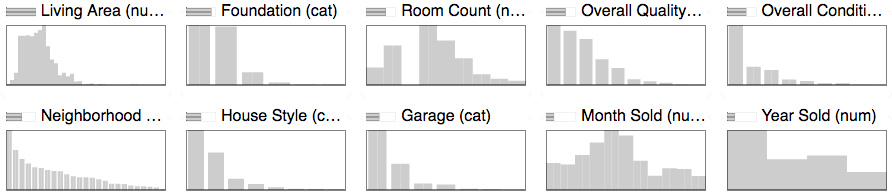
\includegraphics[width=0.41\linewidth]{aggexplain/h_all}}
\raisebox{-0.2\height}{
\parbox{0.16\linewidth}{
\centering
\textsf{$\leftarrow$ Unbiased data set}\\
\textsf{Biased data set $\rightarrow$}\\
\textsf{Compared subset:}\\

\includegraphics[height=1em]{aggexplain/legend_all}
}
}
\raisebox{-0.5\height}{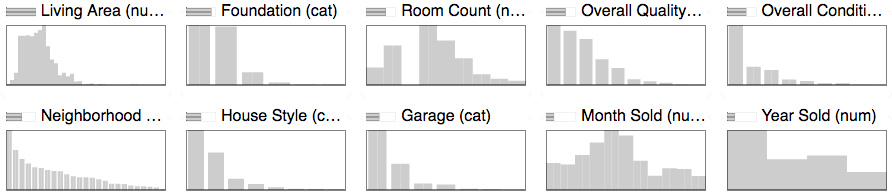
\includegraphics[width=0.41\linewidth]{aggexplain/h_all}}
~\\
\noindent\rule{\linewidth}{0.4pt}
~\\
\raisebox{-0.5\height}{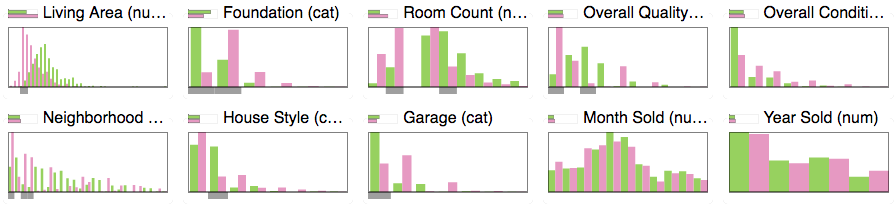
\includegraphics[width=0.41\linewidth]{aggexplain/h_label_ok}}
\raisebox{-0.2\height}{
\parbox{0.16\linewidth}{
\centering
\textsf{$\leftarrow$ Unbiased data set}\\
\textsf{Biased data set $\rightarrow$}\\
\textsf{Compared subset:}\\
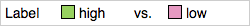
\includegraphics[height=1em]{aggexplain/legend_label}
}
}
\raisebox{-0.5\height}{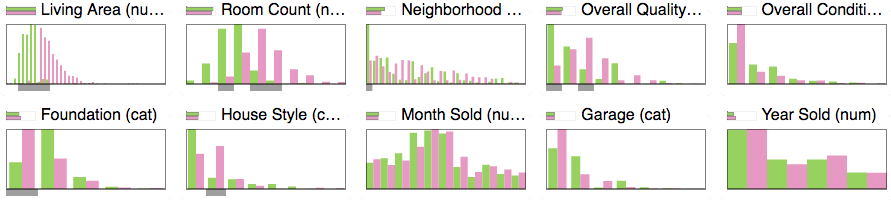
\includegraphics[width=0.41\linewidth]{aggexplain/h_label_bad}}
~\\
\noindent\rule{\linewidth}{0.4pt}
~\\
\raisebox{-0.5\height}{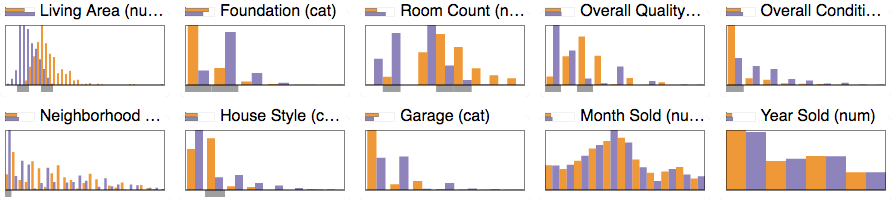
\includegraphics[width=0.41\linewidth]{aggexplain/h_pred_ok}}
\raisebox{-0.2\height}{
\parbox{0.16\linewidth}{
\centering
\textsf{$\leftarrow$ Unbiased data set}\\
\textsf{Biased data set $\rightarrow$}\\
\textsf{Compared subset:}\\
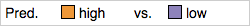
\includegraphics[height=1em]{aggexplain/legend_pred}
}
}
\raisebox{-0.5\height}{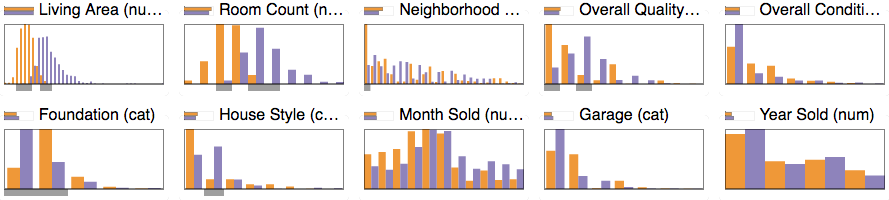
\includegraphics[width=0.41\linewidth]{aggexplain/h_pred_bad}}
~\\
\noindent\rule{\linewidth}{0.4pt}
~\\
\raisebox{-0.5\height}{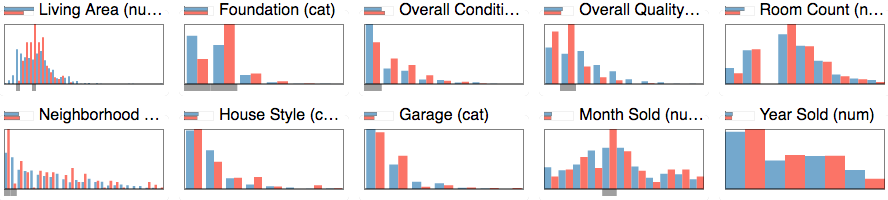
\includegraphics[width=0.41\linewidth]{aggexplain/h_correct_ok}}
\raisebox{-0.2\height}{
\parbox{0.16\linewidth}{
\centering
\textsf{$\leftarrow$ Unbiased data set}\\
\textsf{Biased data set $\rightarrow$}\\
\textsf{Compared subset:}\\

\includegraphics[height=1em]{aggexplain/legend_correct}
}
}
\raisebox{-0.5\height}{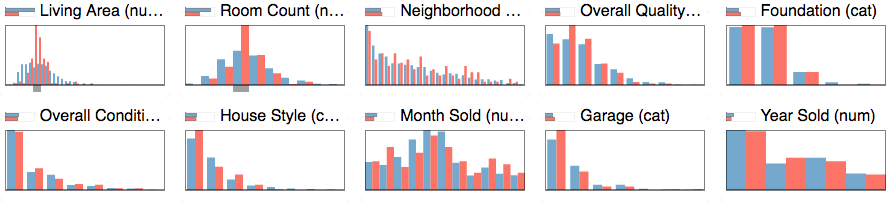
\includegraphics[width=0.41\linewidth]{aggexplain/h_correct_bad}}
\caption{
Comparison of different subset selections on both the unbiased model (left side) and the biased model (right side).
Features are sorted per segment by most important at the top-left, row-wise to least important at the bottom-right.
Note, the feature ``Living Area'', in both the ``Label'' (\ie, ground truth) and ``Pred.'' (\ie, model prediction), has flipped outcomes for the biased model (right side).
Each subset has a different color palette to not confuse different selections with each other.
}
\label{figs:good_vs_bad}
\end{figure*}

\subsection{Study Design}
We study four conditions which result from combining different representations with the inclusion or exclusion of explanations.
The different representations are:

\begin{itemize}
	\item
    A view of the model through individual instances.
    Instances are listed in a table.
    This is an extension of the approach of inspecting instances one-by-one.
    \item
    A view of the model through aggregated instances.
    Instances are aggregated in histograms for individual features.
\end{itemize}

In each of those conditions we compare the ability to detect biases in the data by comparing the unbiased data set to the data set with the manufactured bias.

We also explore the impact of those conditions on whether explanations and aggregation improve trust in the model's decisions.
Particularly, trust in the \emph{right} model.

\subsection{Tasks and Measurements}
In order to test conditions against each other we created a questionnaire.
After asking the participant about the knowledge of machine learning and basic terminology, we have a training section for participants to familiarize themselves with the interface.
First, an introductory video explains all components of the interface.
The video uses an example model from a different data set which is designed to predict whether a room is occupied or not based on predictions from various sensors~\cite{occupancy}.
Then, a series of questions about this example model are asked and the participant can and has to use the interface to answer them correctly.
The questions ask about the values of features under certain conditions, such as ``What is the model's prediction for high values of `$CO_2$?''', ``What is the lowest value of `Humidity' that predicts `occupied'?'', ``Are the predictions for low values of `Light' correct?''.
The questions are constructed in a way to be easily answerable under all conditions given an understanding of the user interface and basic principles of machine learning.
An incorrect answer leads back to the beginning of the section and the participant is given the chance to correct the mistake.
We did not use those questions to exclude any participant but rather for giving them an opportunity to get comfortable with the user interface.
Note, that it is not necessary for participants to have a deep knowledge in \emph{how} machine learning algorithms work, as long as, the basic principles of prediction, ground truth, or accuracy are clear.  This reflects that domain experts would often not necessarily be trained in \emph{developing} machine learning models but rather \emph{using} them.

As final question of this segment the participant has to detect, in a hypothetical, scenario that a prediction does not make \emph{sense} from a semantic standpoint, even though that prediction is \emph{correct} from the perspective of the model.
This question aims to prime the participants for the upcoming task and teaches that model correctness is not necessarily equivalent to semantic correctness.
After this, we ask some common sense questions about how house prices are supposed to correspond to certain features.
This ensures that participants have enough domain knowledge for the upcoming task.

In the main part of the study we present the participant with both housing data models one after the other and encourage them to explore the models with the end goal of determining which model can be trusted more.
The order of the data sets is random.
The participant then has to answer the following questions about each model:
``Do you think the predictions of the model make sense?'',
``How well does the model perform in terms of accuracy?'',
``How much do you trust the model?''
on a five-point Likert scale;
and explain the reasoning for their answers.
For each question we provide a more in-depth explanation with examples.

After inspecting both models, we ask the participants to state which model performs better in terms of accuracy, which model can be trusted more, and whether the model they trust more had the higher or lower accuracy, or no model can be trusted more than the other.
We ask participants to describe their reasoning and also state their confidence in their decision on a five-point Likert scale.

\subsection{Participants}
We ran all four conditions of the study on Prolific\footnote{\url{https://www.prolific.ac/}}, an online survey recruitment system.
Participants in online recruitment aim to increase their payout to effort ratio.
Thus, we took several measures to ensure high data quality.
Firstly, we only allowed participants with a high rating on the platform and an interest in computer science.
Secondly, we excluded all data from participants that had a suspiciously fast completion times (less than 10 minutes after watching the introductory video) which would not allow them to establish well thought out answers.
We also excluded participants with too little interaction with the interface, determined by the number of histograms or table cells they inspected and how often they changed the subset comparison selection.
As attention question we used the question ``Which model had the higher accuracy?'' to remove participants.
This question has an objective answer that had to be determined during the study as well.
By reading the full text answers we could exclude participants that had little understanding of machine learning or the assigned task, or were giving non-sense answers.
We retained 100 eligible participants divided evenly across the four conditions.
This represents less than $47\%$ of total participants, not counting participants that stopped the study before submitting.
